\chapter{CellRouter}
\label{cha:cellrouter}

As explained in the abstract, the aim of this project is to develop divide-and-conquer strategies on a previously existing framework to route standard cells. This router, called CellRouter, uses a technology-independent and parametrizable approach which can be adapted to different fabrics and rules. It uses a boolean formulation of the problem to find a legal detailed routing of a cell represented by a gridded layout. However, as cells become larger, approaches such as the one this project explores become mandatory to keep SAT formulas tractable. In this section, basic insight on how the CellRouter tool works and necessary vocabulary that will later be extensively used is given.\\


\section{The Routing Problem}

As explained in Section \ref{sec:VLSIalg}, routing and manufacturability-aware design have attracted lots of attention in the last years. This routing tool addresses both issues by considering geometrical regularity for the routing process. As mentioned before, it is not the first time that a boolean formulation of the problem is presented \cite{set,vuit}. However, the complexity of the problem restricted the applicability to small cells. Additionally, algorithms based on using regular layout fabrics had already been proposed in \cite{cinc}, but they were specially customized for that fabric and a specific set of design rules. \\

The router we are working on proposes an algorithmic approach for a generic problem of cell routing, which has the following characteristics.

\begin{itemize}
  \item Should be independent from the layout templates and the interconnect resources, so that it can be configured with the resources available at any technology generation.
  \item Attributes should be allowed for every wire segment.
  \item Should allow the router to select the best pin locations.
  \item Should be independent from the set of design rules.
  \item In the case of unroutable cells, externally connected pins should be allowed.
  \item A set of recommended design rules to improve yield should be specifiable.
  \item Wirelength should be a parameter for optimization. \\
\end{itemize} 

To do so, the CellRouter tool uses an encoding scheme for SAT-based formulas that makes large cells tractable by applying windowing heuristics, as explained in Section \ref{sec:satproblems}. A formalism to specify gridded design rules and multiple-patterning constraints is provided. CellRouter also uses heuristics for quality improvement (wirelength and recommended design rules) and allows the connection of external pins in case of unroutability. \\

Graphs are used to represent the gridded routing problem. Every net has a set of terminals that must be connected. Each terminal is represented by a set of vertices.  Edges represent wire segments that can be used to connect pairs of vertices. The routing problem is defined as follows.

\begin{center}\textit{Find a set of edges that define routes connecting the terminals of each net. The routes must be disjoint (cannot have common vertices) and satisfy a set of design rules.}\end{center} 

It is important to realize that the number of possible solutions is finite. It can be reduced to a SAT formula in which a variable is associated to every edge representing the presence or absence of a given signal in that position. To find such a solution with the maximum quality, CellRouter uses two steps.

\begin{enumerate}
  \item Finding a legal solution that honors the design rules.
  \item Improving the solution by iteratively re-routing nets and using quality terms in the cost function.
\end{enumerate}


\section{Routing Problem Representation}

The routing region is represented by a 3D undirected grid graph $G(V,E)$ as depicted in Figure \ref{fig:grid}(a). 

\begin{figure}[h!]
  \centering
  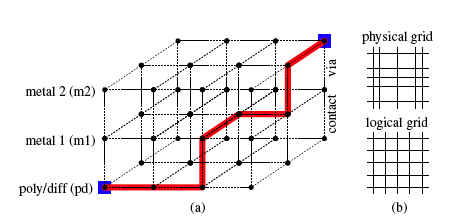
\includegraphics[scale=0.6]{img/bckgrnd/grid.png}
  \caption{(a) Grid model for routing. (b) Physical and logical grid}
  \label{fig:grid}
\end{figure}

The vertices have associated integer coordinates in $\{1, ..., W\} \times \{1, ..., L\} \times \{1, ..., H\}$, where $W$, $L$ and $H$ represent width, length and height. The edges of the graph connect grid points. Notice that the represented physical grid may not have a uniform distribution such as the one shown in the grid as can be seen in Figure \ref{fig:grid}(b). \\

Every vertex $v$ is denoted by its coordinates $v=(x(v),y(v),z(v))$. In our context, $z(v)$ represents the layer of the layout, thus $z(v) \in \{pd, m1, m2\}$ as shown in Figure  \ref{fig:grid}(a). Every edge will be denoted by its endpoints, as in $e(v, u)$. We will also define a \textit{net} $n \subset V$ as a set of grid points, called terminals, that must be connected. A \textit{subnet} will be a pair of terminals of the same net. \\

A Viewer program is provided in order to see how a grid looks like. Given the description of a grid it shows a 3D representation of it using OpenGL, allowing interaction with the model including zoom and rotation. Figure \ref{fig:ANDa} represents an instance of a real routing problem. Each color represents a different net or signal. We can see in the lowest layer some terminals that need to be connected. On the top and bottom of the cell we can see the VDD (voltage, red) and VSS (ground, grey) lines crossing the second layer. On the bottom left side of the screen, a complete list of the signals that appear on the cell is provided.  


\begin{figure}[h!]
  \centering
  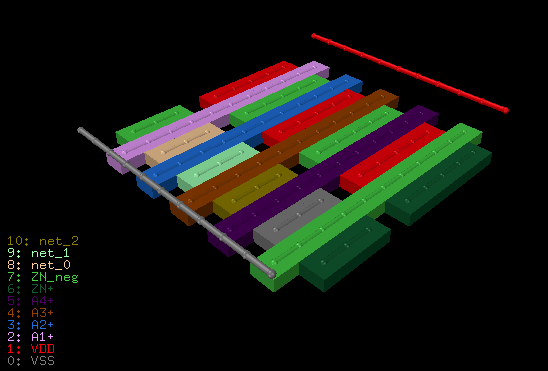
\includegraphics[scale=0.6]{img/bckgrnd/ANDa.png}
  \caption{Routing grid problem instance}
  \label{fig:ANDa}
\end{figure}


\section{SAT to Solve the Routing Problem}
\label{sec:satproblems}

Now that we have some terminology we can make a broad overview at how CellRouter uses SAT to solve the routing problem. To do so, CellRouter codifies the routing problem to a \gls{cnf} formula that can be given as an input to a SAT solver. First, some variables to model the problem are needed.

\begin{itemize}
	\item $\rho(e)$: A variable that represents when edge $e$ is occupied by a wire.
	\item $\rho(e, n)$: A set of variables that represent the associated net in case $e$ is occupied by a wire.
	\item $\rho(e, n, s)$: A set of variables that represent the subnets associated to every wire.
\end{itemize}

Given these variables, the Boolean formula $F$ that represents the problem is as follows.

\begin{center}
$F \equiv C \wedge R \wedge DR$
\end{center}

Here we will have a brief description of the elements in each of the components of $F$.

\begin{description}
  \item[$C$, Consistency constraints] \hfill \\
	These clauses ensure the consistency of the formula. For example, make sure that if an edge is associated with a net, such net is occupied by a wire, or that if an edge is associated to some subnet of a net, it is also associated to that net. 
  
  \item[$R$, Routability constraints] \hfill \\
  	This clause set represents the routing constraints for the grid. For example, we must impose that each edge is assigned to at most one net and that two adjacent wires are assigned to the same net. 
  	
  \item[$DR$, Design-rules contraints] \hfill \\
	Finally, these clauses represent constraints imposed by the user-defined set of design rules. Such design rules might impose, for example, that no adjacent vias can be connected to different nets. Extra clauses modeling wire attributes are included among this constrains.  
	
\end{description}

An important idea which is encoded in the form of routability constraints is windowing. Empirically, it has been shown that the route of a two-terminal subnet rarely spans beyond the bounding box determined by the two terminals. Thus, clauses that enforce the variables outside the region to be falsified can also be added. This might imply that no solution is found even if one exists, but it greatly improves the tractability of the problem. The halo parameter indicates how far outside the bounding box a subnet is allowed to expand. Several halo values will be used in the experiments presented in Chapter \ref{cha:results} \\

CellRouter allows for any discrete set of attributes to be binary-encoded and incorporated to the formula. For example, wires might have two different widths (thin and thick) or could be assigned to different masks to comply with some patterning lithography rules. Additional variables with the form $\rho(e, x)$ which represent the presence of attribute $x$ in edge $e$ are then added, as do the necessary clauses to deal with such attributes. \\

The formula $F$ thus generated is given as an input to the \textit{picosat} SAT solver which will return a satisfying model, if such exists. Given this model, a solution for the original routing problem can be obtained: this is the main goal of the router. In Figure \ref{fig:ANDb} we can see a solution to the routing problem in \ref{fig:ANDa}. \\

\begin{figure}[h!]
  \centering
  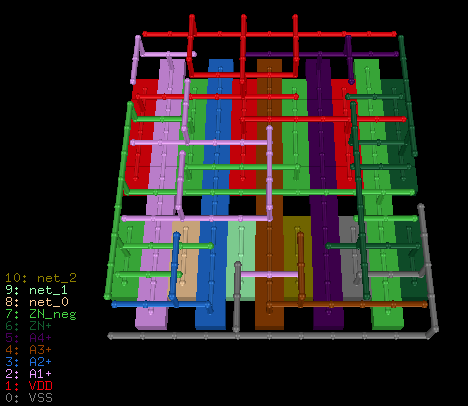
\includegraphics[scale=0.6]{img/bckgrnd/ANDb.png}
  \caption{First obtained solution for \ref{fig:ANDb}}
  \label{fig:ANDb}
\end{figure}


As stated before, among all valid solutions, some have better quality than others. For example, cells with smaller wirelength are preferred. The solution proposed by the SAT solver in \ref{fig:ANDb} has many redundant wires. CellRouter proposes a heuristic method to make this problem tractable using a mixed integer linear programming engine, \textit{gurobi}. However, this model becomes intractable when dealing with large cells. Large neighborhood search is then used to reduce complexity of the problem in combination with \gls{ilp}. The algorithm consists on ripping-up and re-routing nets starting from the basic solution obtained using the SAT solver until no significant improvement is observed. In practice, this takes two rounds of re-routing for each net. This strategy admits variants such as ripping and re-routing more than one net simultaneously; additionally, other aspects such as the ordering of the nets could be considered to search for even better local minima. Figure \ref{fig:ANDc} shows an optimized version of the first obtained solution. \\

\begin{figure}[h!]
  \centering
  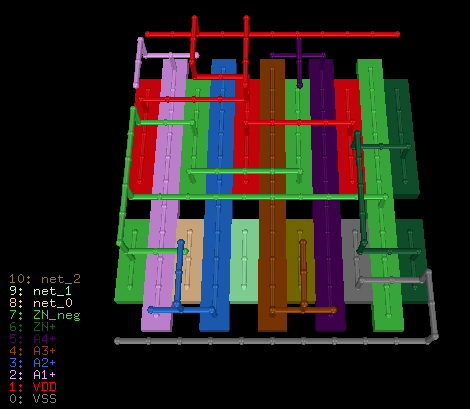
\includegraphics[scale=0.6]{img/bckgrnd/ANDc.png}
  \caption{Optimized solution for \ref{fig:ANDa}}
  \label{fig:ANDc}
\end{figure}

For more information on the grid data structure and what the command line interface of CellRouter is, refer to appendixes \ref{cha:gridformat} and \ref{cha:cli}.

\section{Results}

The CellRouter tool was used to synthesize the Nangate 45nm Open Cell Library, which contains 127 cells. All layouts were checked for design rule correctness and can be found in

\begin{center}
http://layout.potipoti.org
\end{center}

The encoding scheme of CellRouter is compared to another SAT formulation of the routing problem presented in \cite{divuit}. As we can see in Table \ref{tab:tableCellRouter}, CellRouters' $sparse$ encoding outperforms the $dense$ encoding that was used in the previous work. Additionally, it is interesting to see how the windowing heuristic has a big impact on the CPU time for routing cells, managing to divide the computation time at the expenses of losing some solutions. All library cells were routed in 1 hour and 5 minutes. \\

\begin{table}
\centering
\begin{tabular}{lr|rr|rr|rr|}
\cline{3-8}
& & \multicolumn{2}{ c| }{Sparse (w=2)} & \multicolumn{2}{ c| }{Sparse (w=5)} & \multicolumn{2}{ c| }{Dense \cite{divuit}} \\ \cline{1-8}
\multicolumn{1}{|l}{Cell} & Area & Size & CPU & Size & CPU & Size & CPU \\ \cline{1-8}
\multicolumn{1}{|l}{OAI221\_X1} & 5 & 102 & 0.1 & 141 & 0.1 & 96 & 0.1 \\
\multicolumn{1}{|l}{HA\_X1} & 9 & 198 & 0.1 & 249 & 0.1 & 239 & 29.4 \\
\multicolumn{1}{|l}{FA\_X1} & 15 & 521 & 1.2 & 624 & 8.7 & 486 & 2959.0 \\
\multicolumn{1}{|l}{DFFS\_X1} & 21 & 731 & 2.0 & 893 & 8.1 & 903 & 205.4 \\
\multicolumn{1}{|l}{SDFF\_X1} & 25 & 657 & 2.3 & 1073 & 7.2 & 1380 & 1424.0 \\
\multicolumn{1}{|l}{SDFFRS\_X2} & 33 & 1626 & 15.4 & 1944 & 98.1 & 2679 & 40 hours \\ \cline{1-8}
\end{tabular} 
\caption{Results for SAT solving (Size in $10^3$ literals, CPU in secs.)}
\label{tab:tableCellRouter}
\end{table}

However, we must take into account that CellRouter has been applied to cells of a limited size. What happens when it has to deal with bigger, more complex cells? Given that the tool is based on a SAT-solver, and SAT is a hard problem, as soon as the complexity of the problem scales, it becomes intractable. This project aims to find a way for such hard cells to be routed and, to do so, it uses a technique that is not so new in the field of routing algorithms as we have seen in Chapter \ref{cha:background}: The divide-and-conquer approach.


\section{Conclusions}

This chapter has explained the basics of how CellRouter works. First it has more accurately defined what the routing problem for a cell is and how it represents internally the routing grids. Figures of an example of the routing flow have been provided. A basic description of the structure of the SAT formula has also been presented. Finally, origianl times for the CellRouter tool have been provided. Next chapter will focus on how the project uses CellRouter in the process to route bigger and more complex cells, whereas Chapter \ref{cha:partition_strategy} includes the description of the divide-and-conquer techniques used to route such cells.